\section{Resultados Obtidos}

\subsection{Por estados do Brasil}

Na Figura \ref{fig_graf_sigla_uf} abaixo, temos

\begin{figure}[htbp]
	\centerline{
		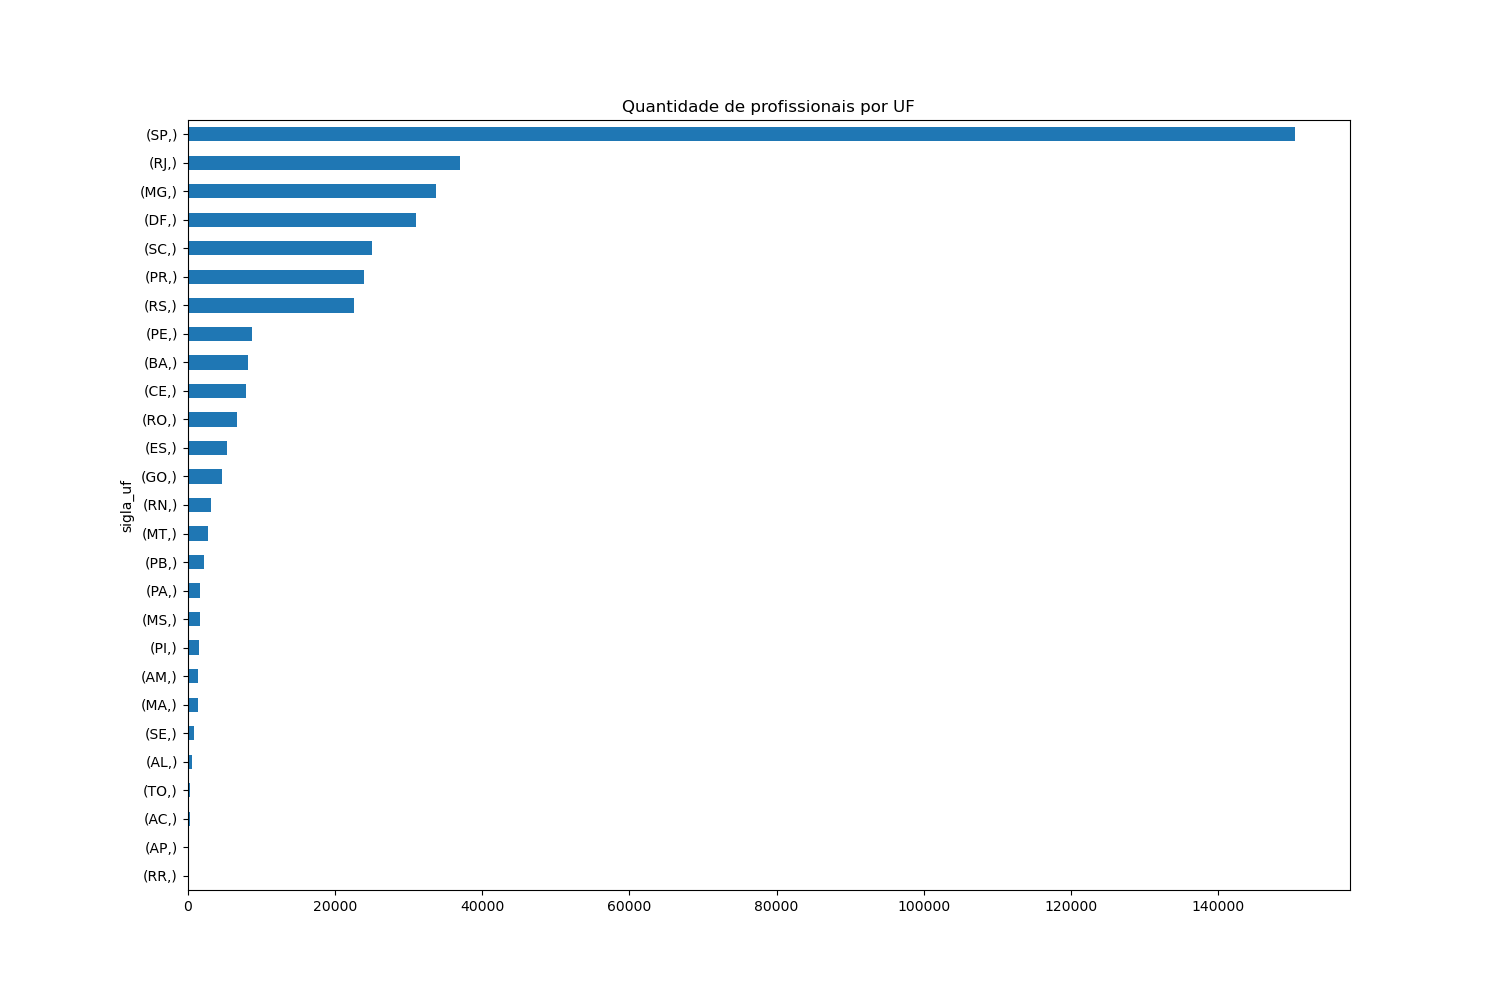
\includegraphics[width=80mm,scale=1]{assets/graf_sigla_uf.png}
	}
	\caption{Quantidade de empregos por estado do Brasil}
	\label{fig_graf_sigla_uf}
\end{figure}

\subsection{Homens X Mulheres}

Na Figura \ref{fig_graf_sexo} abaixo, temos for the same data mining problem. Some techniques have specific requirements regarding the form of the data. Thus, it is often necessary to go back to previous phases to perform adjustments.

\begin{figure}[htbp]
	\centerline{
		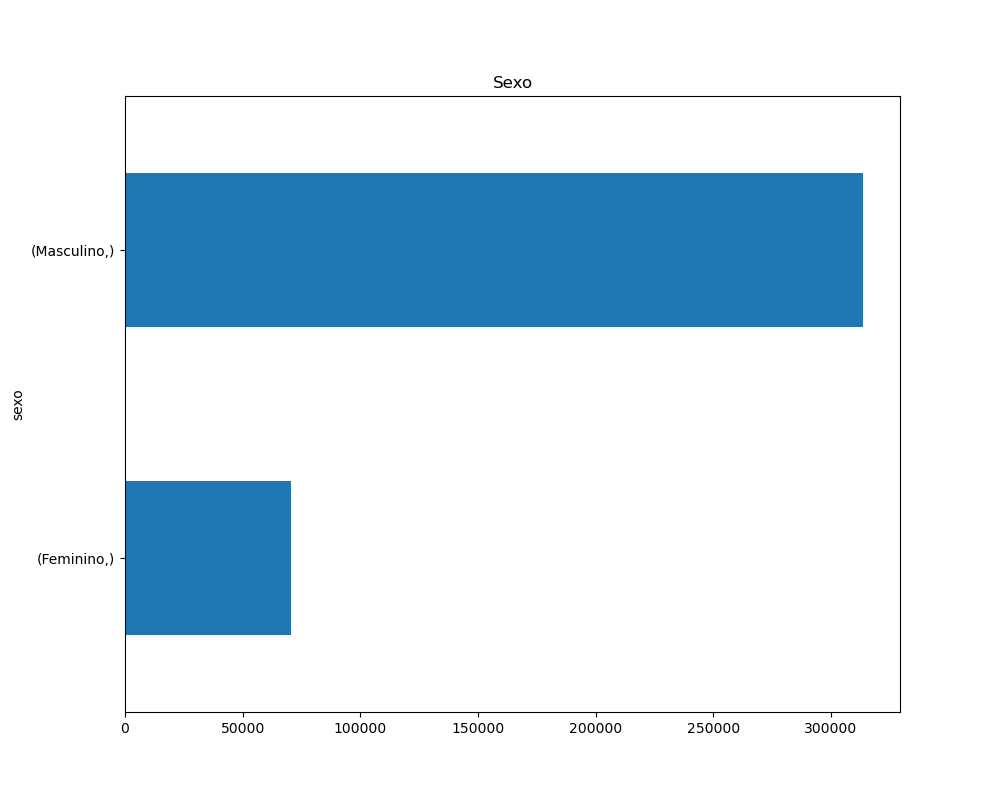
\includegraphics[width=80mm,scale=1]{assets/graf_sexo.png}
	}
	\caption{Quantidade de empregos por gênero}
	\label{fig_graf_sexo}
\end{figure}

\subsection{Por faixa etária}

Neste ponto, verificamos for the same data mining problem. Some techniques have specific requirements regarding the form of the data. Thus, it is often necessary to go back to previous phases to perform adjustments.

\begin{table}[htbp]
	\caption{Comparação CSV vs Parquet}
	\begin{center}
		\begin{tabular}{|c|c|c|c|c|}
			\hline
			\textbf{Arquivo} & \textbf{Gravação} & \textbf{Leitura} & \textbf{Tamanho} \\
			\hline
			CSV              & 106s                & 29s              & 305 mb           \\
			\hline
			Parquet          & 70s                 & 12s              & 329 mb           \\
			\hline
		\end{tabular}
		\label{tab1}
	\end{center}
\end{table}
